\section{Evaluation Details}
\label{app:protocol}

\subsection{Longitudinal inputs and readouts}

The current cohort construction pairs adjacent frontal MIMIC-CXR studies from the same admission, with follow-up intervals of 6--72 hours and requested horizon bins of 6--24 and $>24$--72 hours. Linked MIMIC-IV history is restricted to the source patient and admission, with both event and recording times no later than the source acquisition. The current radiology report is assumed available retrospectively because reliable signing times are unavailable. Future observations supply training targets and scoring references only.

In the completed legacy prototype, a text decoder reads the predicted future state to generate the follow-up report,
and a finding head supplies continuous scores. Forecast training uses 16,000
pairs, validation uses 230, and testing uses 297 pairs from 94 patients. The
full-token, eight-slot, and shuffled-state conditions use Qwen3.5-9B.
All three complete 2,400 forecast updates at effective batch size 32 (seed 42)
from a common newly trained 9B Stage~1 initialization, with metrics and GREEN
scored on all 297 test pairs. The slot adaptation
extracts eight learned queries from the final language layer; the full-token
condition retains valid image/report/history tokens. Both retain the forecast
module. The shuffled condition permutes source states across patients.
It generates one unique report across all 297 pairs, compared with 224 for
slots and 287 for full-token. These adaptations are separate from the proposed
multi-depth $4+4$ design; archived 0.8B scores do not populate their rows.

\paragraph{Unified joint-training protocol (evaluation pending).}
The maintained Qwen3.5-0.8B implementation constructs four JEPA--language
fusion slots and four native-vision slots, each of width 1024. The temporal
branch reads source images and reports, with signed elapsed time supplied only
to the predictor; it does not read EHR variables. The report decoder receives
projected predicted slots and a fixed prompt, and the finding head reads the
predicted state. The true follow-up supplies detached EMA state targets and
report/finding supervision only. Encoder and report-decoder LoRA parameters
are independent, while immutable pretrained language weights share storage.

A single optimizer jointly trains the online encoder, predictor, and active
task heads from the first update. Each update combines one temporal batch with
one current-task batch, cycling through classification, report generation,
segmentation, and SR. The current-task loss has weight 1; future latent,
report, and finding losses have weights 1, 1, and 0.5. Current-task inputs
withhold the same-exam report, and both SR input branches use only LR imagery.
The optional visual consistency objective has weight 0.1 on spatial tasks.
The target encoder copies the online encoder at initialization and follows
EMA with momentum 0.99 after every optimizer update.

The maintained configuration specifies an eight-hour continuous budget on
four GPUs, with per-rank batches of 16 current observations and 32 directed
temporal pairs and accumulation 1. This gives global batch sizes of 64 and
128; capacity and full-run execution remain to be verified. Training starts
from the original pretrained backbones. Historical staged checkpoints do not
initialize this run, and no historical scores are reassigned to the joint
model. Four current tasks are implemented; full six-task evaluation remains
pending.

Matched native supervised, current-slot, full-token, and shuffled-state
comparisons remain to be completed. Controls sharing the encoders and decoder
are needed to separate the effects of temporal prediction and state compression
from the additional JEPA feature pathway.

BioViL-T and CheXWorld freeze their official visual encoders and train shared
evidence fusion, forecast modules, and readouts with the same forecast budget.
They inherit the common V-JEPA-derived Stage~1 warm start, with visual adapters
reinitialized for their feature dimensions; they are adaptations, not native
forecast systems from the original papers. The public VLM rows use zero-shot
forecast prompts, with Qwen3.5-9B as the Qwen checkpoint. Permitted evidence and
references are shared, but training regimes, pretraining data, parameter counts,
and actual GPU hours differ. Nominal model sizes do not denote total system
parameters. Results are single-seed point estimates; paired uncertainty estimates
remain to be computed.

Copy Current repeats the source report and represents persistence for progression
scoring; historical comparisons in that report are not reinterpreted as new
changes after the source time. It has no continuous-score interface. The
finding-transition prior fits future-finding probabilities on the 16,000 training
pairs with fixed Laplace smoothing ($\alpha=1$), conditional on the prepared
source finding label and horizon, with a horizon-specific marginal fallback for
unknown source labels. Its structured source annotations are a privileged
source-status interface and are not VLM predictions. AP, AUROC, Brier, and ECE
are complete; threshold selection and transition scoring remain pending. It has
no severity-direction or free-form report output.

\subsection{Future-prediction metrics}

Table~\ref{main-tab:future_prediction} fixes four dimensions with two metrics each. The current finding schema covers atelectasis, cardiomegaly, consolidation, edema, pleural effusion, and pneumothorax. A frozen CheXbert extractor maps reference and generated reports to findings. Reference labels that are uncertain or unmentioned are masked; predictions cannot reduce the evaluation mask. Each metric reports its reference-defined support and coverage, shared across methods.

\paragraph{Future clinical status.}
Finding AP is the macro average of non-interpolated average precision; AUROC is also computed per finding and macro-averaged. Both use continuous scores and the same set of findings with positive and negative reference support. Class prevalence and eligible counts accompany the results.

For a zero-shot VLM, each finding is queried independently with the same source evidence and horizon. If $\ell_{\mathrm{yes}}$ and $\ell_{\mathrm{no}}$ are the conditional log-likelihoods of fixed candidate answers, the score is $s=\exp(\ell_{\mathrm{yes}})/(\exp(\ell_{\mathrm{yes}})+\exp(\ell_{\mathrm{no}}))$. Single-token candidates use next-token logits; multi-token candidates use complete answer log-likelihoods at a fixed answer boundary. Both candidates must be scored, even if one is absent from an API's top-$k$ output. These ranking scores need not be calibrated clinical probabilities. Prompts, tokenization, masks, and parsing are fixed before test evaluation. Trained forecasters instead use a supervised finding head; the new native supervised and state-augmented conditions will share that readout and its supervision. Comparisons with archived zero-shot Yes/No scores therefore retain a different probability source and do not isolate state conditioning.

\paragraph{Disease progression.}
Transition F1 treats onset ($0\rightarrow1$) and resolution ($1\rightarrow0$) as separate events for each finding. Both source and future references must be assessable. Stable cases remain in the evaluation and can contribute false-positive changes; an omitted finding does not count as a correctly predicted resolution. F1 is computed for each finding--event pair and averaged over pairs with reference-positive event support. This is an event-level macro average, not a pooled micro F1 or an unweighted average of the onset and resolution subgroup means.

Direction F1 assesses improved, stable, and worsened findings on reference-defined pairs where the abnormality persists at both endpoints and its direction is assessable. Annotations identify the finding, laterality, and comparison anchored to the selected source study; conflicting or unanchored reference comparisons are ineligible. Left and right changes are scored separately when annotated, and overlapping whole-patient and side-specific annotations are not counted twice. F1 is macro-averaged over supported finding--scope--direction classes. Missing predictions, incorrect resolutions, and parsing failures remain errors on the fixed eligible references. Equal coarse severity bins alone do not establish stability. The direction annotation vocabulary, reference review, and supported scopes will be frozen before model comparison; this label validation remains pending for the 297-pair cohort. Scores from a separate 82-pair direction study with a different input protocol are not inserted into the main table.

\paragraph{Future report fidelity.}
RadGraph uses the RadGraph-XL partial F1 variant, averaged over reports. GREEN~\citep{ostmeier2024green} assesses clinical content errors using a frozen evaluator. The target Findings/Impression scope, scorer checkpoints, prompts, and failure handling are fixed across methods before evaluation. These scores measure agreement with observed follow-up reports; source-anchored changes are evaluated separately by the progression metrics.

\paragraph{Probabilistic reliability.}
The same future-finding scores used for AP/AUROC are evaluated as probability predictions. For finding $k$ with fixed valid reference set $\mathcal I_k$, the Brier score is $|\mathcal I_k|^{-1}\sum_{i\in\mathcal I_k}(p_{ik}-y_{ik})^2$, macro-averaged over the common finding set. It measures overall probability error, including both discrimination and calibration. Classwise ECE uses ten fixed equal-width probability bins for each finding: it sums the absolute difference between the mean predicted positive probability and observed positive fraction within each bin, weighted by the bin's share of valid references, then macro-averages across findings. Empty bins contribute zero. This adapts binned calibration evaluation~\citep{guo2017calibration} to per-finding event probabilities rather than top-label confidence. Lower Brier and ECE are better.

The main table evaluates uncalibrated probability predictions. Metric definitions
and archived values retain their original scale; Tables~\ref{main-tab:future_prediction}
and~\ref{main-tab:downstream_tasks} display scores multiplied by 100, except PSNR
(dB), with two decimal places. Any post-hoc calibration will be fitted using validation data only, with a matched calibration procedure across methods, and reported separately. Reliability diagrams, bin counts, and horizon-specific comparisons remain planned supplementary analyses. These metrics assess the selected follow-up cohort and report-derived references, not unrestricted population disease risk.

\paragraph{Supplementary analyses.}
The supplementary analysis plan includes separate onset and resolution F1,
stable-reference false-change rates, direction confusion matrices, horizon
breakdowns, and paired patient-bootstrap intervals; not all are complete.
CheXbert macro-positive F1 and future retrieval remain supplementary. Planned
Future R@1 ranks the actual follow-up and fixed other-patient candidates by
disagreement with a common predicted finding schema, extracted from reports or
emitted by the transition prior. Candidates must be matched on horizon,
acquisition conditions, coarse current findings, and reference assessability;
ties split first-place credit equally. Candidate-pool size and eligible-query
counts will accompany retrieval scores. Degree errors require reviewed ordinal
annotations. These analyses do not add columns to the fixed eight-metric table.

\subsection{Downstream supervision}

The joint model uses eight $1024$-dimensional slots: four from vision--language fusion layers and four from the VLM's native vision encoder. Each source contributes an early layer, two intermediate layers, and its final layer through learned aggregation and projection. Classification and report generation read all eight slots; segmentation and SR read only $S_{5:8}$ together with the task image, which is LR for SR. Task gradients jointly train the slot readouts and decoders. This construction differs from the initial last-layer-slot prototype and requires new training. The expanded six-task evaluation adds standard VQA and phrase grounding; all image-based current tasks withhold the same-exam report.

Classification uses 13 report-derived finding/device labels, excluding No Finding,
and masks uncertain or missing labels. The test set has 353 images; macro ranking
metrics include the 11 labels with positive and negative support. DINOv2 and
CheXWorld classification heads use 13,681 training images, 160 validation images,
and 20 epochs. Their stored \texttt{macro\_auprc} field implements
non-interpolated average precision. Current-report scoring uses 507 images and
withholds the target Findings/Impression. Standard VQA is planned on
MIMIC-CXR-VQA with its full answer ontology, negative examples, and empty answer
sets. Official Accuracy and micro F1 will be supplemented by question-type and
region breakdowns. MS-CXR phrase grounding requires fixed heatmap-to-box
conversion, multi-box matching, and invalid-output treatment. Derived
disease-list QA and Chest ImaGenome anatomical-region localization are not
substitutes for those benchmarks. Benchmark test patients must be excluded from
all current-task and temporal training sources; available public-checkpoint pretraining
overlap remains to be documented.

Segmentation uses quality-filtered CXAS pseudo-labels for the two lungs and heart,
with 4,096/249/447 training/validation/test images. Human Dice separately measures
the two lungs on 138 Montgomery images, without a heart label. SR uses the same
CXR split and antialiased bicubic downsampling by four per spatial dimension,
with HR long edge capped at 512 pixels. Every image input receives LR for SR;
HR supplies supervision only. Padding is excluded from losses and image metrics.
The dense-task rows use 20 epochs, effective batch size eight, and seed 20260913.

Qwen3.5-9B visual-slot rows freeze the native vision encoder and train a task
decoder conditioned on four multi-depth visual slots. Their shuffled control
permutes these conditions across patients; the image-only decoder uses zero
context. These rows do not use the eight-slot forecast pilot or full language
model. DINOv2/CheXWorld freeze spatial encoders and train the same pixel-task
decoder; their spatial-token counts differ from the four-slot interface.
SwinIR-M uses public DF2K $4\times$ pretraining and adapts all 11.9 million
parameters to the CXR degradation. Matching data and epochs does not match
compute: SwinIR consumes 8.313 GPU hours including evaluation, versus 0.161 for
the image-only SR run on the same GPU model. MAIRA-2 retains its native
report/grounding interface, but its results are pending.

The planned no-slots baseline and full \method{} will share six-task supervision
and decoder budgets; those rows remain TBD. Earlier report-assisted scores,
$2\times$ SR, and separate two-epoch joint dense-task pilots are excluded.
\pending{complete full six-task adaptation, official VQA and MS-CXR grounding,
and cross-task exclusion/pretraining-overlap audits for
Table~\ref{main-tab:downstream_tasks}}.

\begin{figure*}[p]
    \centering
    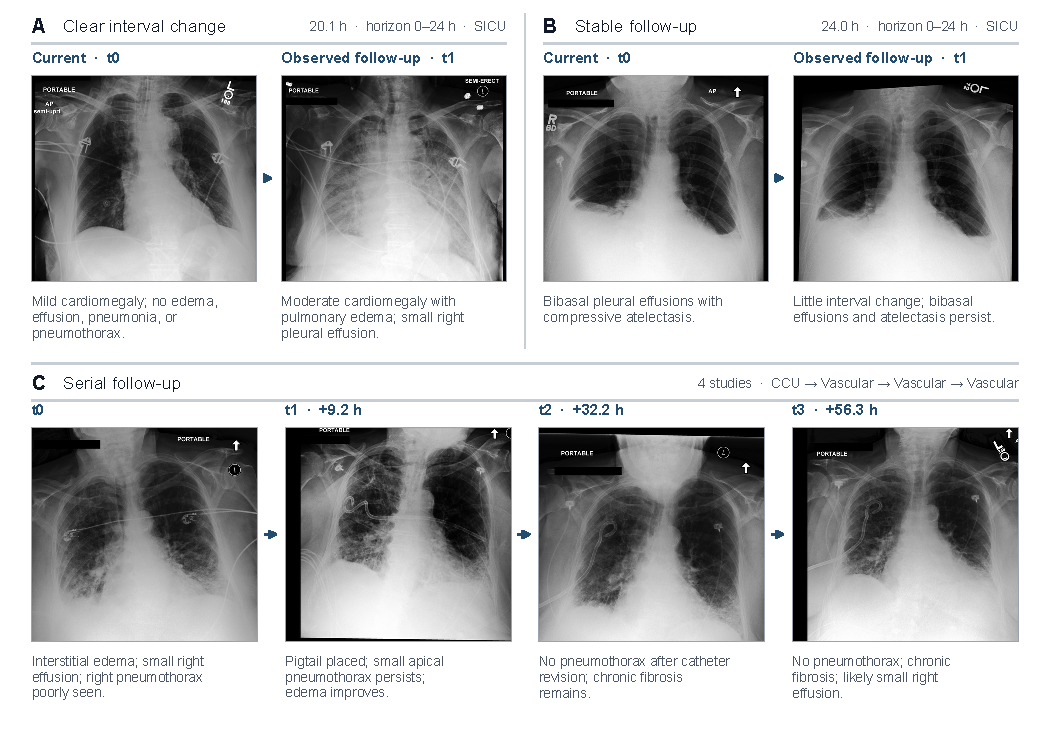
\includegraphics[width=0.90\textwidth,height=0.82\textheight,keepaspectratio]{ppt/ppt/appendix_fig1_v1.pdf}
    \caption{Representative longitudinal MIMIC-CXR trajectories. Cases A and B show paired current and follow-up radiographs with elapsed times and report summaries, illustrating interval change and stability, respectively. Case C shows four serial examinations over 56.3 hours. These examples show observed images and report summaries, not model predictions.}
    \label{fig:appendix_mimic_longitudinal_cxr}
\end{figure*}
